\section{Circuiti dinamici in regime transitorio}
Ci occupiamo in questa sezione dell'analisi di circuiti dinamici in regime transitorio.
\begin{dfn}[Circuito dinamico]
	Un circuito è detto dinamico quando contiene almeno un componente dinamico.
	Si definisce \textit{ordine del circuito} il numero di componenti dinamici presenti nel circuito. L'ordine del circuito determina il comportamento generale del circuito.
\end{dfn}
\begin{dfn}[Regime transitorio]
		Il \textit{regime transitorio} è l'evoluzione temporale di $v(t),\ i(t)$ che si osserva tra una condizione di regime stazionario/periodico e un'altra. Sapendo studiare queste fasi, si ha un'idea del comportamento di un circuito in tutti gli istanti del suo utilizzo, che è prevalentemente stazionario o periodico, e in cui le fasi transitorie sono dovute all'accensione, allo spegnimento, o al cambiamento di topologia del circuito, ad esempio tramite l'attivazione di interruttori.
\end{dfn}
\subsection{Circuiti dinamici di ordine 1}
\subsubsection{Circuito RC - Evoluzione libera}
Consideriamo un circuito come in \cref{fig:rclibera}, in cui:
\begin{itemize}
	\item $t<0:\quad v_C=V_0, \frac{d}{dt}v_C=0$;
	\item $t = 0$: commutazione interruttore.
\end{itemize}
\begin{figure}[H]
	\centering
	\includegraphics[width=0.7\linewidth]{rclibera}
	\caption{Circuito i riferimento per lo studio del transitorio di un circuito RC. Il condensatore viene caricato per $t<0$ e lasciato scaricare successivamente, grazie alla commutazione degli interruttori.}
	\label{fig:rclibera}
\end{figure}

Per la proprietà di continuità della tensione osservata per il condensatore, 
\[\begin{aligned}
	v_C(0^-) = v_C(0^+) = V_0\\
	Q_C(0^-) = Q_C(0^+) = CV_0\\
	E_C(0^-) = E_C(0^+) = \frac{1}{2}CV_0^2
\end{aligned}\]
Studiamo dunque ciò che avviene per $t \geq  0$, quando si innesca un regime transitorio (di scarica, come vedremo in seguito).
\begin{figure}
	\centering
	\includegraphics[width=0.7\linewidth]{rclibera1}
	\caption{Schema del circuito RC con versi di riferimento (VDR) assegnati al fine di effettuare i calcoli necessari}
	\label{fig:rclibera1}
\end{figure}
Facendo riferimento ai VDR in \cref{fig:rclibera1}, osserviamo che:
\[LKT:\ v_R(t) + v_C(t) = 0 \]
\[R i_R(t) + v_C(t) = 0\]
\[LKC:\ i_R(t) = i_C(t) = C \frac{dv_C(t)}{dt}\]
Dunque otteniamo l'equazione differenziale di primo grado lineare omogenea:
\[RC\frac{dv_C(t)}{dt} + v_C(t) = 0\]
Integrando tramite il metodo di separazione delle variabili
\[\int_{v_C(0)}^{v_C(t)} \frac{dv_C}{v_C} = -int_0^t \frac{dt}{RC}\]
si ottiene:
\[\left[ ln|v_C|\right ]_{v_C(0)}^{v_C(t)} = -\frac{t}{RC}\]
Da cui, con pochi semplici passaggi algebrici, si giunge all'equazione dell'evoluzione libera (o \textit{evoluzione naturale}) di $v_C$:
\[v_C(t) = V_0 e^{-\frac{t}{RC}}\]
\[v_C(t) = \begin{cases}
				&V_0,\quad \qquad t<0\\
				&V_0 e^{-\frac{t}{RC}}, \quad t\geq0
\end{cases}
\]
Questo andamento è descritto graficamente in \cref{fig:rcliberagrafico}:
\begin{figure}[H]
	\centering
	\begin{tikzpicture}[>=latex, thick, scale=1.2]
		% Definizioni per personalizzare il grafico
		\def\Vzero{2.5} % Altezza del valore V0 sull'asse y
		\def\ttau{1.0}   % Costante di tempo per il decadimento esponenziale
		
		% --- Assi ---
		% Asse orizzontale (Tempo t)
		\draw[->] (-2.5, 0) -- (8, 0) node[right] {$t$};
		% Asse verticale (Tensione v_C(t))
		\draw[->] (0, -0.5) -- (0, 3.5) node[above] {$v_C(t)$};
		
		% --- Etichette ---
		% Etichetta per l'origine t=0
		\node[below] at (0, -0.4) {$t=0$};
		% Etichetta per il valore iniziale V0
		% Disegna un piccolo tratto sull'asse y e posiziona l'etichetta
		\draw (0.1, \Vzero) -- (-0.1,\Vzero) node[above=3pt,left] {$V_0$};
		
		% --- Curva ---
		% Parte 1: Tensione costante per t < 0
		\draw[blue, thick] (-2.5, \Vzero) -- (0, \Vzero);
		
		% Parte 2: Decadimento esponenziale per t >= 0
		% La funzione plotteggiata è V0 * exp(-t/tau)
		\draw[blue,  thick, domain=0:7.8, samples=100, smooth] 
		plot (\x, {\Vzero * exp(-\x/\ttau)});
		% Linea tratteggiata verticale da t=tau alla curva
		\draw[dashed] (\ttau, 0) -- (\ttau, {\Vzero * exp(-1)});
		% Tick e etichetta sull'asse
		\draw (\ttau, 0.1) -- (\ttau, -0.1) node[below] {$\tau$};
		
		% Tick e etichetta sull'asse
		\draw (5*\ttau, 0.1) -- (5*\ttau, -0.1) node[below] {$5\tau$};
	\end{tikzpicture}
	\label{fig:rcliberagrafico}
	\caption{Evoluzione temporale libera della tensione in un circuito RC in regime transitorio}
\end{figure}
Notiamo in particolare che gli unici parametri che influenzano la risposta sono $V_0$ e $RC$. Con $RC$ maggiore, $\frac{t}{RC}$ diminuisce e la risposta è più lenta; e viceversa. Vista l'importanza di $RC$, che è definito dalle caratteristiche dei componenti circuitali scelti. Vista l'importanza di questo termine, la definiamo \textit{costante di tempo} del circuito: 
\[tau = RC (s)\] 
Tramite una semplice analisi dimensionale è possibile verificare che il prodotto $RC$ è una quantità di tempo, e si misura in secondi.\\
$v_c(t=\infty)= 0$. Ci chiediamo però dopo quanto tempo possiamo considerare il transitorio approssimativamente concluso. Notiamo innanzitutto che in un tempo $\tau$ la tensione si riduce di circa il 63\% (vedi \cref{fig:rcliberagrafico}).
\[v_C(\tau) = V_0 e^{-\frac{t}{\tau}} = \frac{V_0}{e} \approx 0,37V_0\] 
Notiamo anche che:
\[v_C(5\tau)<1\% V_0\]
Dunque possiamo considerare il transitorio concluso approssimativamente dopo un tempo di $5\tau$.\\

Similmente, possiamo indagare l'andamento della corrente nel tempo.
\[i_C(t) = C\frac{dv_C(t)}{dt} \Rightarrow C\frac{d}{dt} (V_0e^{-\frac{t}{\tau}}) = C(-\frac{1}{\tau}) V_0e^{-\frac{t}{\tau}} = (-\frac{V_0}{R})e^{-\frac{t}{\tau}} = -I_0e^{-\frac{t}{\tau}} = -\frac{v_C(t)}{R}\]
L'andamento della corrente nel tempo durante il transitorio è dunque rappresentata in \cref{fig:rcliberagrafico1}. Notiamo la discontinuità della corrente: questo è l'esito dell'idealità del circuito, con induttanza nulla. Per circuiti reali, con componenti induttiva non nulla, per quanto minima, si avrà una salita della corrente molto rapida, ma non nettamente discontinua come rappresentata nel grafico.

\begin{figure}[H]
	\centering
	\begin{tikzpicture}[>=latex, thick, scale=1.2]
		% Definizioni per personalizzare il grafico
		\def\Izero{1.25} % Altezza del valore V0 sull'asse y
		\def\ttau{1.0}   % Costante di tempo per il decadimento esponenziale
		
		% --- Assi ---
		% Asse orizzontale (Tempo t)
		\draw[->] (-2.5, 0) -- (8, 0) node[right] {$t$};
		% Asse verticale (Corrente v_C(t))
		\draw[->] (0, -2.0) -- (0, 3.5) node[above] {$i_C(t)$};
		
		% --- Etichette ---
		% Etichetta per l'origine t=0
		\node[left] at (0, 0.4) {$t=0$};
		% Etichetta per il valore iniziale V0
		% Disegna un piccolo tratto sull'asse y e posiziona l'etichetta
		\draw (0.1, -\Izero) -- (-0.1,-\Izero) node[below=3pt,right] {$I_0 = -V_0/R$};
		
		% --- Curva ---
		% Parte 1: Tensione costante per t < 0
		\draw[orange, thick] (-2.5, 0) -- (0, 0);
		
		% Parte 2: Decadimento esponenziale per t >= 0
		% La funzione plotteggiata è V0 * exp(-t/tau)
		\draw[orange,  thick, domain=0:7.8, samples=100, smooth] 
		plot (\x, {-\Izero * exp(-\x/\ttau)});
		% Linea tratteggiata verticale da t=tau alla curva
		\draw[dashed] (\ttau, 0) -- (\ttau, {-\Izero * exp(-1)});
		% Tick e etichetta sull'asse
		\draw (\ttau, 0.1) -- (\ttau, -0.1) node[above=3pt] {$\tau$};
		
		% Tick e etichetta sull'asse
		\draw (5*\ttau, 0.1) -- (5*\ttau, -0.1) node[above=3pt] {$5\tau$};
	\end{tikzpicture}
	\label{fig:rcliberagrafico1}
	\caption{Evoluzione temporale libera della corrente attraverso il resistore (nonché attraverso il capacitora) di un circuito RC in regime transitorio}
\end{figure}
Osserviamo il bilancio energetico durante il transitorio. Verifichiamo la conservazione dell'energia durante il transitorio.
\[p_{A,C} (t) = v_C(t) i_C(t) = -\frac{V_0^2}{R} e^{-\frac{2t}{\tau}}\]
\[p_{A,R} (t) = v_R(t) i_R(t) = \frac{V_0^2}{R} e^{-\frac{2t}{\tau}}\]
\begin{itemize}
	\item La potenza erogate dal condensatore, nonché assorbita dal resistore, è un esponenziale negativo. Notiamo che la costante di tempo dell'andamento della potenza è dimezzata rispetto a quella dell'evoluzione della corrente e della tensione.
	\item Il condensatore assorbe una potenza negativa, ossia eroga potenza; il resistore assorbe una potenza positiva. Risulta dunque che C alimenta R durante il transitorio, fino a quando non esaurisce l'energia che aveva immagazzinato in precedenza, nella condizione di $v_C = V_0$.
\end{itemize}
Estendiamo il ragionamento al calcolo delle energie scambiate durante il transitorio.
\[E_{A,R}(t) = \int_0^t p_{A,R}(t)dt = \frac{V_0^2}{R}\int_0^t e^{-\frac{2t}{\tau}}dt = \frac{V_0^2C}{2}\left[ e^{\frac{-2t}{\tau}}\right]_0^t = -\frac{CV_0^2}{2}(e^{\frac{-2t}{\tau}} - 1) = \frac{CV_0^2}{2}(1- e^{\frac{-2t}{\tau}})\]
Osserviamo, per completezza:
\[E_{A,R}(0) = 0\]
\[E_{A,R}(\infty) = \frac{CV_0^2}{2}\]
Dunque all'istante iniziale, il resistore è ancora a tensione nulla, perciò non assorbe energia. Osserviamo invece che, dopo tempo infinito, tutta l'energia immagazzinata nel condensatore al tempo $t=0$ viene dissipata dal resistore.

\subsubsection{Circuito RL - Evoluzione libera}
Seguiamo un procedimento analogo per studiare un circuito RL in evoluzione libera.
Consideriamo un circuito come in \cref{fig:rllibera}, in cui:
\begin{itemize}
	\item $t<0:\quad v_L= L\frac{di_L}{dt} = 0$;
	\item $t = 0$: commutazione interruttore.
\end{itemize}
Affinché l'induttore venga caricato, deve essere connesso a un generatore di corrente per $t<0$
\begin{figure}[H]
	\centering
	\includegraphics[width=0.7\linewidth]{rllibera}
	\caption{Circuito i riferimento per lo studio del transitorio di un circuito RL. L'induttore viene caricato per $t<0$ e lasciato scaricare successivamente, grazie alla commutazione degli interruttori.}
	\label{fig:rllibera}
\end{figure}

Per la proprietà di continuità della corrente osservata per l'induttore, 
\[\begin{aligned}
	i_L(0^-) = i_L(0^+) = I_0\\
	\Phi_L(0^-) = \Phi_L(0^+) = Li_L\\
	E_L(0^-) = E_L(0^+) = \frac{1}{2}LI_0^2
\end{aligned}\]


Studiamo dunque ciò che avviene per $t \geq0$, quando si innesca un regime transitorio di scarica.
\begin{figure}[H]
	\centering
	\includegraphics[width=0.7\linewidth]{rllibera1}
	\caption{Schema del circuito RL con versi di riferimento (VDR) assegnati al fine di effettuare i calcoli necessari}
	\label{fig:rllibera1}
\end{figure}
Facendo riferimento ai VDR in \cref{fig:rllibera1}, osserviamo che:
\[LKC :\ i_R(t) + i_L(t) = 0 \]
\[\frac{v_L(t)}{R} + i_L= 0\]
\[v_L(t) = L \frac{d}{dt} i_L(t)\]
Dunque otteniamo l'equazione differenziale di primo grado lineare omogenea:
\[\frac{L}{R}\frac{di_L(t)}{dt} + i_L(t) = 0\]
Notando l'analogia con l'equazione già risolta per il circuito RC in evoluzione libera, si ottiene direttamente
\[i_L(t) = I_0 e^{-\frac{t}{\tau}}\]
in cui, in questo caso, $\tau = \frac{R}{L}$\footnote{Anche in questo caso è possibile verificare che questa quantità ha le unità di misura di un tempo tramite una semplice analisi dimensionale} è la \textit{costante di tempo} del circuito RL. Questo circuito ha quindi un comportamento duale a quello del circuito RC, nel senso che il comportamento della corrente di questo è analogo a quello della tensione dell'altro (\cref{fig:rlliberagrafico}), e viceversa.
\begin{figure}[H]
	\centering
	\begin{tikzpicture}[>=latex, thick, scale=1.2]
		% Definizioni per personalizzare il grafico
		\def\Izero{2.5} % Altezza del valore V0 sull'asse y
		\def\ttau{1.0}   % Costante di tempo per il decadimento esponenziale
		
		% --- Assi ---
		% Asse orizzontale (Tempo t)
		\draw[->] (-2.5, 0) -- (8, 0) node[right] {$t$};
		% Asse verticale (Corrente i_L(t))
		\draw[->] (0, -0.5) -- (0, 3.5) node[above] {$i_L(t)$};
		
		% --- Etichette ---
		% Etichetta per l'origine t=0
		\node[below] at (0, -0.4) {$t=0$};
		% Etichetta per il valore iniziale I0
		% Disegna un piccolo tratto sull'asse y e posiziona l'etichetta
		\draw (0.1, \Izero) -- (-0.1,\Izero) node[above=3pt,left] {$I_0$};
		
		% --- Curva ---
		% Parte 1: Tensione costante per t < 0
		\draw[orange, thick] (-2.5, \Izero) -- (0, \Izero);
		
		% Parte 2: Decadimento esponenziale per t >= 0
		% La funzione plotteggiata è V0 * exp(-t/tau)
		\draw[orange,  thick, domain=0:7.8, samples=100, smooth] 
		plot (\x, {\Izero * exp(-\x/\ttau)});
		% Linea tratteggiata verticale da t=tau alla curva
		\draw[dashed] (\ttau, 0) -- (\ttau, {\Izero * exp(-1)});
		% Tick e etichetta sull'asse
		\draw (\ttau, 0.1) -- (\ttau, -0.1) node[below] {$\tau$};
		
		% Tick e etichetta sull'asse
		\draw (5*\ttau, 0.1) -- (5*\ttau, -0.1) node[below] {$5\tau$};
	\end{tikzpicture}
	\label{fig:rlliberagrafico}
	\caption{Evoluzione temporale libera della corrente in un circuito RL in regime transitorio}
\end{figure}
L'andamento della tensione nel circuito RL può essere ricavato facilmente:
\[v_L(t) = \begin{cases}
	&0 ,\quad \qquad t<0\\
	&L \frac{di_L}{dt} = L \frac{1}{\tau}I_0 e^{-\frac{t}{\tau}} = -R I_0 e^{-\frac{t}{\tau}} = -R i_L(t), \quad t\geq0
\end{cases}
\]
Questo andamento è graficato in \cref{fig:rlliberagrafico1}
\begin{figure}[H]
	\centering
	\begin{tikzpicture}[>=latex, thick, scale=1.2]
		% Definizioni per personalizzare il grafico
		\def\Vzero{1.25} % Altezza del valore V0 sull'asse y
		\def\ttau{1.0}   % Costante di tempo per il decadimento esponenziale
		
		% --- Assi ---
		% Asse orizzontale (Tempo t)
		\draw[->] (-2.5, 0) -- (8, 0) node[right] {$t$};
		% Asse verticale (Tensione v_L(t))
		\draw[->] (0, -2.0) -- (0, 3.5) node[above] {$v_L(t)$};
		
		% --- Etichette ---
		% Etichetta per l'origine t=0
		\node[left] at (0, 0.4) {$t=0$};
		% Etichetta per il valore iniziale V0
		% Disegna un piccolo tratto sull'asse y e posiziona l'etichetta
		\draw (0.1, -\Vzero) -- (-0.1,-\Vzero) node[below=3pt,right] {$V_0 = -RI_0$};
		
		% --- Curva ---
		% Parte 1: Tensione costante per t < 0
		\draw[blue, thick] (-2.5, 0) -- (0, 0);
		
		% Parte 2: Decadimento esponenziale per t >= 0
		% La funzione plotteggiata è V0 * exp(-t/tau)
		\draw[blue,  thick, domain=0:7.8, samples=100, smooth] 
		plot (\x, {-\Vzero * exp(-\x/\ttau)});
		% Linea tratteggiata verticale da t=tau alla curva
		\draw[dashed] (\ttau, 0) -- (\ttau, {-\Vzero * exp(-1)});
		% Tick e etichetta sull'asse
		\draw (\ttau, 0.1) -- (\ttau, -0.1) node[above=3pt] {$\tau$};
		
		% Tick e etichetta sull'asse
		\draw (5*\ttau, 0.1) -- (5*\ttau, -0.1) node[above=3pt] {$5\tau$};
	\end{tikzpicture}
	\label{fig:rlliberagrafico1}
	\caption{Evoluzione temporale libera della tensione sull'induttore di un circuito RL in regime transitorio}
\end{figure}
Anche in questo caso, in maniera duale al precedente, la discontinuità nella tensione è dovuta all'ipotesi ideale di capacità nulla nel circuito.
Anche relativamente al bilancio energetico, valgono considerazioni  e risultati analoghi a quelli mostrati per il circuito RC.

\subsubsection{RC - Evoluzione forzata}
Consideriamo il circuito in \cref{fig:rcforzata}, costituito da un generatore collegato in serie a un interruttore, un resistore e un condensatore carico.
\begin{figure}[H]
	\centering
	\includegraphics[width=0.7\linewidth]{rcforzata}
	\caption{Circuito RC con generatore indipendente di tensione costante, con VDR di tensioni e correnti per riferimento per i calcoli successivi}
	\label{fig:rcforzata}
\end{figure}

Per $t<0$, l'interruttore è aperto, con $v_C(0) = 0$ e $\frac{d}{dt} v_C(t) = 0$. A $t = 0$ si verifica la commutazione dell'interruttore. Ci proponiamo di studiare il transitorio del condensatore. Ci aspettiamo in ogni caso che per $t = \infty$, cioè a transitorio concluso, $v_C(\infty) = V_g$. È possibile trarre questa conclusione dal fatto che la corrente sul condensatore $i_C (\infty) = C\frac{dv_C}{dt}(\infty) = 0$ quando si raggiunge nuovamente un regime stazionario, in cui la tensione ai capi del condensatore non varia. Essendo $v_R(\infty) = R i_R (\infty)= 0$, risulta necessariamente $v_C(\infty) = V_g$.

Considerando i VDR in \cref{fig:rcforzata},
\[LKT:\ V_g = v_R(t) + v_C(t)\]
\[V_g = R i(t) + v_C(t)\]
\[RC \frac{dv_C}{dt} + v_C(t) = V_g\]
Otteniamo dunque un'equazione differenziale lineare di primo grado, a coefficienti costanti, non omogenea, che può ancora una volta essere risolta per separazione delle variabili:
\[\int_{v_C(0)=V_0}^{v_C(t)} \frac{dv_C}{V_g - v_C(t)} = \int_0^t \frac{dt}{RC}\]
\[ln\left(\frac{|v_C - V_g|}{|V_0 - V_g|}\right) = -\frac{t}{RC}\]
\[v_C(t) = V_g + (V_0 - V_g)e^{-\frac{t}{RC}} \]
Notiamo che $\lim{t \to \infty} v_C(t) = V_g$, coerentemente con le nostre considerazioni preliminari. Notiamo anche che, ancora una volta coerentemente con le ipotesi iniziali:
\[v_C(0) = V_0\]
Per visualizzare graficamente l'andamento della tensione nel tempo durante l'evoluzione forzata, notiamo innanzitutto che i parametri che possono essere modificati "da progettisti" per determinare il comportamento del circuito sono $V_0$, $V_g$ e $\tau = RC$. L'andamento della tensione è rappresentato in \cref{fig:rcforzatagrafico}. Notiamo che il caso particolare per $V_g = 0,\ V_0>0$ corrisponde all'evoluzione libera.

\begin{figure}[H]
	\centering
	% --- PRIMO GRAFICO (SINISTRA) ---
	% Larghezza 0.45 per lasciare spazio al centro
	\begin{subfigure}{0.45\linewidth} 
		\centering
		% \resizebox{larghezza}{altezza}{contenuto}
		% "!" mantiene le proporzioni dell'altezza automaticamente
		\resizebox{\linewidth}{!}{%
			\begin{tikzpicture}[>=latex, thick] % Rimosso 'scale', ci pensa resizebox
				\def\Vzero{1.0}
				\def\ttau{1.0}
				\def\Vg{2.5}
				
				\draw[->] (-2.5, 0) -- (8, 0) node[right] {$t$};
				\draw[->] (0, -0.5) -- (0, 3.5) node[above] {$v_C(t)$};
				
				\node[below] at (0, -0.4) {$t=0$};
				\draw (0.1, \Vzero) -- (-0.1,\Vzero) node[above=3pt,left] {$V_0$};
				\draw (0.1, \Vg) -- (-0.1,\Vg) node[above=3pt,left] {$V_g$};
				
				\draw[blue, thick] (-2.5, \Vzero) -- (0, \Vzero);
				\draw[blue, thick, domain=0:7.8, samples=100, smooth] 
				plot (\x, {\Vg +(\Vzero - \Vg) * exp(-\x/\ttau)});
				
				\draw[dashed] (\ttau, 0) -- (\ttau, {\Vg +(\Vzero - \Vg)* exp(-1)});
				\draw[dashed] (0, \Vg) -- (7.8, \Vg);
				\draw (\ttau, 0.1) -- (\ttau, -0.1) node[below] {$\tau$};
				
				\draw (5*\ttau, 0.1) -- (5*\ttau, -0.1) node[below] {$5\tau$};
				\draw[dashed] (5*\ttau, 0) -- (5*\ttau, {\Vg +(\Vzero - \Vg)* exp(-5)});
			\end{tikzpicture}%
		} % Fine resizebox
		\caption{$V_g > V_0$}
	\end{subfigure}
	\hfill % Spazio elastico che riempie il buco (circa 10% della pagina)
	% --- SECONDO GRAFICO (DESTRA) ---
	\begin{subfigure}{0.45\linewidth}
		\centering
		\resizebox{\linewidth}{!}{%
			\begin{tikzpicture}[>=latex, thick]
				\def\Vzero{2.5} 
				\def\ttau{1.0}
				\def\Vg{1.0}
				
				\draw[->] (-2.5, 0) -- (8, 0) node[right] {$t$};
				\draw[->] (0, -0.5) -- (0, 3.5) node[above] {$v_C(t)$};
				
				\node[below] at (0, -0.4) {$t=0$};
				\draw (0.1, \Vzero) -- (-0.1,\Vzero) node[above=3pt,left] {$V_0$};
				\draw (0.1, \Vg) -- (-0.1,\Vg) node[above=3pt,left] {$V_g$};
				
				\draw[blue, thick] (-2.5, \Vzero) -- (0, \Vzero);
				\draw[blue, thick, domain=0:7.8, samples=100, smooth] 
				plot (\x, {\Vg +(\Vzero - \Vg) * exp(-\x/\ttau)});
				
				\draw[dashed] (\ttau, 0) -- (\ttau, {\Vg +(\Vzero - \Vg)* exp(-1)});
				\draw[dashed] (0, \Vg) -- (7.8, \Vg);
				\draw (\ttau, 0.1) -- (\ttau, -0.1) node[below] {$\tau$};
				
				\draw (5*\ttau, 0.1) -- (5*\ttau, -0.1) node[below] {$5\tau$};
				\draw[dashed] (5*\ttau, 0) -- (5*\ttau, {\Vg +(\Vzero - \Vg)* exp(-5)});
			\end{tikzpicture}%
		} % Fine resizebox
		\caption{$V_g < V_0$}
	\end{subfigure}
	
	\caption{Andamento della tensione sul condensatore di un circuito RC in regime transitorio in evoluzione forzata}
	\label{fig:rcforzatagrafico}
\end{figure}
\subsubsection{Scomposizione della risposta di circuiti del primo ordine ed evoluzione forzata di un circuito RL}
Possiamo vedere la risposta $v_C(t) = V_g + (V_0 - V_g) e^{-\frac{t}{\tau}}$ come composta da:
\begin{itemize}
	\item una risposta a regime: $v_{C,r} = V_g$, ossia una parte permanente;
	\item una risposta transitoria: $v_{C, t} (t) = (V_0 - V_g) e^{-\frac{t}{\tau}}$. Questa può anche essere chiamata \textit{risposta temporanea}, perché si esaurisce con il passare del tempo: $v_{C,t} (\infty) = 0$.
\end{itemize}
Notiamo che, noto il valore di $\tau$, bastano due informazioni per determinare $v_C(t)$, ossia $v_C(0) = V_0$ e $v_C(\infty) = V_g$. 
\[v_C(t) = v_{C,t} (t) + v_{C,r} = [v_C(0) - v_C(\infty)] e^{-\frac{t}{\tau}} + v_C(\infty)\]
Dunque, siccome abbiamo osservato che il circuito RL ha un comportamento duale a quello del circuito RC,
\[i_L(t) = i_{L,t} (t) + i_{L,r} = [i_L(0)- i_L(\infty)]e^{-\frac{t}{\tau}} + i_L(\infty)\]
In sintesi, possiamo concludere che la risposta completa di un circuito del $\mathrm{1^\circ}$ ordine dipende da:
\begin{itemize}
	\item [1. ] Valore \textbf{iniziale} della variabile di stato ($v_C(0)$ o $i_L(0)$)
	\item [2. ] Valore \textbf{finale} della variabile di stato ($v_C(\infty)$ o $i_L(\infty)$)
	\item [3. ] Costante di tempo $\tau$ ($\tau_C = RC$ o $\tau_L = \frac{L}{R}$)
\end{itemize}

\begin{ex}
	Determinare $i_L(t)$ durante il transitorio nel circuito in \cref{fig:exrlforz}
	\begin{figure}[H]
		\centering
		\includegraphics[width=0.7\linewidth]{exrlforz}
		\caption{}
		\label{fig:exrlforz}
	\end{figure}
	Sarebbe possibile risolvere questo esercizio anche usando le leggi di Kirchhoff e risolvendo le equazioni differenziali risultanti. Tramite la scomposizione della risposta, tuttavia, è possibile pervenire più rapidamente al una soluzione.
	\[i_L(t) = [i_L(0) - i_L(\infty)] e^{-\frac{t}{\tau}} + i_L(\infty)\]
	\[\tau = \frac{L}{R}\]
	Studiamo poi il circuito a $t = 0^-$, in regime stazionario con interruttore aperto: siccome il ramo contenente l'induttore è aperto,
	\[i_L (0^-) = 0\]
	Per un'analisi in più passaggi, si può prima osservare che l'induttore in regime stazionario si comporta come un cortocircuito, e dunque sostituirlo nel circuito dato con tale componente, per poi notare che, con l'interruttore aperto, su di esso non scorre alcuna corrente.
	Per le proprietà di continuità della corrente sull'induttore, poi, 
	\[i_L (0^+) = i_L(0^-) = i_L(0) = 0\]
	Determiniamo infine $i_L(\infty)$. Notiamo che a $t=\infty$, si avrà interruttore chiuso e il transitorio sarà concluso, e si sarà instaurato un nuovo regime stazionario, diverso da quello iniziale. Nuovamente, si può considerare l'induttore come un cortocircuito e calcolare la corrente che vi scorre attraverso, ossia la risposta a regime, come:
	\[i_L(\infty) = \frac{V_g}{R}\]
	Perciò,
	\[i_L(t) = [0 - \frac{V_g}{R}] e^{-\frac{Rt}{L}} + \frac{V_g}{R} = \frac{V_g}{R}(1- e^{-\frac{Rt}{L}})\]
	
\end{ex}
Notiamo che per la risoluzione di un circuito dinamico del primo ordine in regime transitorio è necessario risolvere due circuiti in regime stazionario, uno per $t=0$ e uno per $t=\infty$.
Per un circuito del primo ordine generale, cioè con un solo componente dinamico connesso a una rete complessa di componenti non dinamici, è possibile ottenere direttamente la soluzione tramite l'individuazione del circuito equivalente di Thevenin o Norton. Come abbiamo visto, i due teoremi sono sostanzialmente equivalenti, e si può dimostrare che portano alla stessa soluzione per questi circuiti, grazie alle relazioni $R_T = R_N$ e $V_T = R_T I_N$.
Tuttavia, per comodità nel calcolo e nell'analisi del circuito, spesso può essere conveniente utilizzare:
\begin{itemize}
	\item l'equivalente Thevenin se il componente dinamico collegato è un condensatore ($\tau = R_T C$);
	\item l'equivalente Norton se il componente dinamico collegato è un induttore ($\tau = \frac{L}{R_N}$)
\end{itemize}
\subsection{Circuiti dinamici di ordine 2}
Per la definizione di ordine, questi circuiti contengono due componenti dinamici. Questi circuiti corrispondono al caso reale, in quanto è impossibile, nella realtà, avere un circuito con induttanza o capacità davvero nulla. Questi circuiti portano a equazioni differenziali di secondo ordine per la risoluzione del loro transitorio. Esistono due tipi di circuiti di questo tipo, denominati \textit{RLC serie} e \textit{RLC parallelo}, in cui \textit{serie} e \textit{parallelo} sono riferiti al tipo di collegamento tra i componenti L e C (\cref{fig_confRLC}). 
\begin{figure}
	\centering
	\includegraphics[width=0.5\linewidth]{confrlc}
	\caption{Confronto tra i due tipi generali di circuiti del secondo ordine. A sinistra, RLC serie; a destra, RLC parallelo.}
	\label{fig:confrlc}
\end{figure} 
Analogamente ai circuiti del primo ordine, trovare una soluzione generale a questi due tipi di circuito permette di risolvere tutti i circuiti del secondo ordine, a seguito di opportune semplificazioni circuitali.

\subsubsection{RLC serie - Evoluzione libera}
Consideriamo, ad esempio, un circuito come in \cref{fig:rlcsl}, che rappresenta il caso realistico in cui il transitorio è innescato dalla chiusura di un interruttore. Altri scenari possibili potrebbero essere più complicati.
\begin{figure}[H]
	\centering
	\includegraphics[width=0.7\linewidth]{rlcsl}
	\caption{}
	\label{fig:rlcsl}
\end{figure}

Per $t = 0^-$, il circuito è in regime stazionario, con interruttore aperto, e $i_L (0^-) = I_0$, $v_C(0^-) = V_0$. Notiamo che non è possibile che scorra una corrente sull'induttore in questa configurazione, ma seguiamo una trattazione generale con $I_0$ non necessariamente nulla per dare una soluzione più generale del transitorio.\\
Al tempo $t=0$ si chiude l'interruttore e si innesca il transitorio.\\
A $t=0^+$, grazie alle proprietà di continuità delle variabili di stato sui nostri componenti dinamici, sappiamo che $i_L(0^+)=i_L (0^-) = I_0$ e $v_C(0^+) = v_C(0^-) = V_0$. Ci proponiamo dunque di studiare il comportamento del circuito per $t \geq 0$ (\cref{fig:rlcsl1}).
\begin{figure}[H]
	\centering
	\includegraphics[width=0.7\linewidth]{rlcsl1}
	\caption{}
	\label{fig:rlcsl1}
\end{figure}
\[LKT:\ v_R(t) + v_L(t) + v_C(t) = 0\]
Utilizzando le leggi costitutive e notando che la corrente che attraversa i tre componenti, collegati in seri, è la stessa,
\[R i(t) + L\frac{di}{dt} + \frac{1}{C}\int_{0^+}^t i dt = 0\]
\[R \frac{di}{dt} + L\frac{d^2i}{dt^2} + \frac{1}{C}i(t) = 0\]
\begin{equation} \label{eq:rlc}
	\frac{d^2i}{dt^2} + \frac{R}{L}\frac{di}{dt} + \frac{1}{LC} i(t) = 0
\end{equation}
Si ottiene dunque un'equazione differenziale ordinaria lineare di ordine 2, a coefficienti costanti, omogenea.
Le condizioni iniziali necessarie alla risoluzione del problema di Cauchy associato a questa equazione differenziale ordinaria sono:
\begin{enumerate}
	\item $i (0^+) = i_L (0^+) = I_0$
	\item $\left. \frac{di}{dt} \right |_{0^+} = \left. \frac{di_L}{dt} \right |_{0^+}$, la quale deve essere ricavata dallo studio del circuito a $t = 0^+$. Siccome $v_L = L \frac{di_L}{dt}$, $\frac{di_L}{dt} = \frac{v_L}{L}$. Per determinare $v_L(0^+)$ utilizziamo già ora un metodo generale, poi utilizzabile anche negli esercizi. Per $t = 0+$, si possono considerare il condensatore come un generatore indipendente di tensione ($V_0$) e l'induttore come un generatore indipendente di corrente ($I_0$), che possiamo comunque descrivere tramite la convenzione dell'utilizzatore (\cref{fig:rlcsl2}).
	\begin{figure}[H]
		\centering
		\includegraphics[width=0.7\linewidth]{rlcsl2}
		\caption{Circuito RLC serie semplificato a $t=0^+$ tramite le condizioni iniziali per ricavare $v_L (0^+)$}
		\label{fig:rlcsl2}
	\end{figure}
	\[v_L (0^+) = - (v_R (0^+) + V_0) = -(RI_0 + V_0)\]
	Perciò,
	\[ \left. \frac{di}{dt} \right |_{0^+} = -\frac{RI_0 + V_0}{L}\] 
\end{enumerate}
Procediamo dunque alla risoluzione dell'equazione differenziale associata al sistema (\cref{eq:rlc}), con polinomio caratteristico 
\[\lambda^2 + \frac{R}{L}\lambda + \frac{1}{LC} = 0\]
\[\lambda_{1,2} = \frac{R}{2L} \pm \sqrt{(\frac{R}{2L})^2 - \frac{1}{LC}}\]. 
Chiamiamo:
\begin{itemize}
	\item $\lambda_{1,2}$ \textit{frequenze naturali} del circuito, perché rappresentano la frequenza dell'oscillazione dell'esponenziale complesso (o sinuosoide) che rappresenta la soluzione, come si vedrà in seguito, e hanno dimensioni di una frequenza fisica (Hz);
	\item $\alpha = \frac{R}{2L}$ \textit{fattore di smorzamento}, per le ragioni che saranno chiare con la risoluzione;
	\item $\omega_0 = \frac{1}{\sqrt{LC}}$ \textit{pulsazione di risonanza}, in continuità con quanto è possibile osservare dall'analisi di circuiti LC, in particolare per quanto riguarda la frequenza di risonanza del circuito.
\end{itemize}
Il polinomio caratteristico assume quindi la forma
\[\lambda^2 + 2 \alpha + \omega_0^2 = 0\]
E le soluzioni (con $\Delta = \alpha^2 - \omega_0^2$):
\[\lambda_{1,2} = -\alpha \pm \sqrt{\alpha^2 - \omega_0^2} = -\alpha \pm \sqrt{\Delta}\]
Le soluzioni possibili in base ai valori dei parametri sono:
\begin{enumerate}
	\item $\Delta > 0$ (\textit{Risposta sovrasmorzata});
	\item $\Delta = 0$ (\textit{Risposta smorzata critica});
	\item $\Delta < 0$ con $\alpha > 0$ (\textit{Risposta sottosmorzata});
	\item $\Delta < 0$ con $\alpha = 0$ (\textit{Risposta senza smorzamento}).
\end{enumerate}
Procediamo dunque ad analizzarle in dettaglio:
\begin{enumerate}
	\item \textit{Risposta sovrasmorzata}\\
		$\Delta > 0 \Leftrightarrow \alpha > \omega_0$, ossia fattore di smorzamento maggiore della pulsazione di risonanza.\\
		Osserviamo che questo caso si verifica per valori della resistenza grandi relativamente a capacità e induttanza.
		\[\lambda_{1,2} = -\alpha \pm \sqrt{\Delta} \in \mathbb{R} < 0\]
		La soluzione è dunque del tipo
		\[i(t) = A_1 e^{\lambda_1t} + A_2 e^{\lambda_2t}\]
		con $A_1,\ A_2$ (in questo caso così come nei successivi) parametri costanti che dipendono dalle soluzioni iniziali. Osserviamo che la soluzione ha una forma analoga a quella vista per circuiti del primo ordine, con esponenziali negativi (con forma variabile in base ai valori dei due parametri).
		\[i(0) = A_1 + A_2\]
		Notiamo anche che $\tau = - \frac{1}{\lambda}$. Un possibile andamento è rappresentato in \cref{fig:sovra}. In generale, comunque, lo smorzamento è rapido, e dominato dall'esponenziale più lento, e si può osservare al massimo un estremante relativo (massimo o minimo, il base ai valori relativi di $A_1,\ A_2,\ \lambda_1,\ \lambda_2$).
		\begin{figure}[H]
			\centering
			\begin{tikzpicture}[>=latex, thick, scale=1.2]
				% Definizioni per personalizzare il grafico
				\def\Auno{1.5} 
				\def\Adue{-2.5}
				\def\Tuno{1.5}
				\def\Tdue{0.5}
				
				% --- Assi ---
				% Asse orizzontale (Tempo t)
				\draw[->] (-1.5, 0) -- (8, 0) node[right, above = 3 pt] {$t$};
				% Asse verticale (Corrente i_L(t))
				\draw[->] (0, -3.5) -- (0, 2.5) node[above] {$i(t)$};
				
				% --- Etichette ---
	
				\draw (0.1, \Auno) -- (-0.1,\Auno) node[above=3pt,left] {$A_1$};
				\draw (0.1, \Adue) -- (-0.1,\Adue) node[above=3pt,left] {$A_2$};
				\draw (0.1, \Auno + \Adue) -- (-0.1,\Auno + \Adue) node[above=3pt,left] {$A_1 + A_2$};
				
				% --- Curva ---
				
				% La funzione plotteggiata è V0 * exp(-t/tau)
				\draw[orange!30,  thick, domain=0:7.8, samples=100, smooth] 
				plot (\x, {\Auno * exp(-\x/\Tuno)});
				\draw[orange!30,  thick, domain=0:7.8, samples=100, smooth] 
				plot (\x, {\Adue * exp(-\x/\Tdue)});
				\draw[orange,  thick, domain=0:7.8, samples=100, smooth] 
				plot (\x, {\Adue * exp(-\x/\Tdue) + \Auno * exp(-\x/\Tuno)});
				% Linea tratteggiata verticale da t=tau alla curva
				%\draw[dashed] (\ttau, 0) -- (\ttau, {\Izero * exp(-1)});
				% Tick e etichetta sull'asse
				%\draw (\ttau, 0.1) -- (\ttau, -0.1) node[below] {$\tau$};
				
				% Tick e etichetta sull'asse
				%\draw (5*\ttau, 0.1) -- (5*\ttau, -0.1) node[below] {$5\tau$};
			\end{tikzpicture}
			\label{fig:sovra}
			\caption{}
		\end{figure}
	\item \textit{Risposta smorzata critica}\\
		$\Delta = 0 \Leftrightarrow \alpha = \omega_0$, ossia fattore di smorzamento uguale alla pulsazione di risonanza.\\
		\[\lambda_1 = \lambda_2 = -\alpha \in \mathbb{R} < 0\]
		La soluzione è dunque del tipo
		\[i(t) = (A_1 + A_2t) e^{-\alpha t}\]
		Notiamo che uno dei due parametri pre-esponenziali è moltiplicato per un termine lineare ($t$). Il comportamento sarà dunque simile a quello precedente, ma con specificità da questo termine, che declina più lentamente dell'altro. 
		Nell'andamento di $i(t)$ può essere presente un massimo (o un minimo, in base ai valori dei parametri) anche più grande (in valore assoluto) della corrente $I_0$ o del valore iniziale, a un istante $\tau_M$ (\cref{fig:critica}), il che può essere un vantaggio o una minaccia per il corretto funzionamento o l'integrità del circuito. Questa è la risposta non oscillatoria che arriva a regime più velocemente, perciò è indicato per circuiti in cui è necessario un transitorio breve, ma in cui non può essere accettata una risposta oscillatoria.
		\[i(0) = A_1\]
		Determiniamo il tempo al quale si verifica il massimo valore della corrente, calcolando la derivata e trovando l'istante in cui si annulla:
		\[\frac{d}{dt} [(A_1 + A_2t) e^{-\alpha t}] = (-\alpha A_1 e^{-\alpha t}-\alpha A_2t e^{-\alpha t} +  A_2e^{-\alpha t}\]
		\[\tau_M = \frac{A_2 - \alpha A_1}{\alpha A_2} = \frac{1}{\alpha} - \frac{A_1}{A_2}\]
		\begin{figure}[H]
			\centering
			\begin{tikzpicture}[>=latex, thick, scale=1.2]
				% Definizioni per personalizzare il grafico
				\def\Auno{-1.5} 
				\def\Adue{2.0}
				\def\alfa{1.0}
				\pgfmathsetmacro\tm{1/\alfa - \Auno/\Adue}
				
				% --- Assi ---
				% Asse orizzontale (Tempo t)
				\draw[->] (-1.5, 0) -- (8, 0) node[right, above = 3 pt] {$t$};
				% Asse verticale (Corrente i_L(t))
				\draw[->] (0, -3.5) -- (0, 2.5) node[above] {$i(t)$};
				
				% --- Etichette ---
				
				\draw (0.1, \Auno) -- (-0.1,\Auno) node[above=3pt,left] {$A_1$};
				\draw (0.1, \Adue) -- (-0.1,\Adue) node[above=3pt,left] {$A_2$};
				\draw (0.1, \Auno + \Adue) -- (-0.1,\Auno + \Adue) node[above=3pt,left] {$A_1 + A_2$};
				
				% --- Curva ---
				
				\draw[orange!30,  thick, domain=0:7.8, samples=100, smooth] 
				plot (\x, {\Auno * exp(-\x *\alfa)});
				\draw[orange!30,  thick, domain=0:7.8, samples=100, smooth] 
				plot (\x, {\Adue *\x * exp(-\x *\alfa)});
				\draw[orange,  thick, domain=0:7.8, samples=100, smooth] 
				plot (\x, {\Adue *\x * exp(-\x *\alfa) + \Auno * exp(-\x *\alfa)});
				% Linea tratteggiata verticale da t=tau alla curva
				\draw[dashed] (\tm, 0) -- (\tm, {\Adue *\tm * exp(-\tm *\alfa) + \Auno * exp(-\tm *\alfa)} );
				% Tick e etichetta sull'asse
				\draw (\tm, 0.1) -- (\tm, -0.1) node[left, below] {$\tau_M$};
				
				% Tick e etichetta sull'asse
				%\draw (5*\ttau, 0.1) -- (5*\ttau, -0.1) node[below] {$5\tau$};
			\end{tikzpicture}
			\label{fig:critica}
			\caption{}
		\end{figure}
	\item \textit{Risposta sottosmorzata}\\
	$\Delta < 0\ (\alpha >0)\ \Leftrightarrow \alpha < \omega_0$, ossia fattore di smorzamento minore alla pulsazione di risonanza, con fattore di smorzamento comunque positivo.\\
	Detto $\beta = \sqrt{-\Delta}$,
	\[\lambda_{1,2} = -\alpha \pm j \beta \in \mathbb{C}\]
	Dunque $\lambda_{1,2}$ sono complesse coniugate (come previsto dal corollario del Teorema Fondamentale dell'Algebra).
	La soluzione è dunque del tipo
	\[i(t) = e^{-\alpha t} [A_1cos(\beta t) + A_2sin(\beta t)]\] 
	Detti $A = \sqrt{A_1^2 + A_2^2}$ e $\phi = -atan\left(\frac{A_2}{A_1}\right)$, si può scrivere in maniera equivalente
	\[i(t) = Ae^{-\alpha t} cos(\beta t + \phi)\]
	\[i(0) = Acos\phi\]
	L'andamento è del tipo indicato in \cref{fig:sottosmorzata}, è cioè una risposta oscillante smorzata con andamento esponenziale.
	\begin{itemize}
		\item Ha tempo caratteristico unico $\tau = \frac{1}{\alpha}$;
		\item ha frequenza di oscillazione $f= \frac{\beta}{2\pi}$ e quindi periodo $T = \frac{2 \pi}{\beta}$;
		\item è la risposta che tende a regime più velocemente in assoluto. 
		\item ha primo massimo o minimo con valore assoluto piuttosto alto, ed è quindi una risposta "violenta". Per questo è ad esempio utilizzata nelle candele dei motori a benzina, per innescare la combustione, dove il circuito ha smorzamento basso, per garantire scariche forti ripetute nel tempo.
		\item Questa è la risposta che decade più velocemente all'interno della fascia di tolleranza, per valori di $\alpha$ minori di $\omega_0$ ma \textit{sufficientemente grandi}, anche se la risposta smorzata critica è quella che decade più rapidamente asintoticamente \footnote{
			\begin{enumerate}
				\item Dimostrazione del decadimento asintotico.
				Si dimostra che, a parità di pulsazione naturale $\omega_0$, la risposta critica si assesta asintoticamente più rapidamente. 
				Siano $i_{crit}(t) = (A_1 + A_2 t)e^{-\omega_0 t}$ la risposta critica e $E_{sotto}(t) = A e^{-\alpha t}$ l'inviluppo della risposta sottosmorzata (con $0 < \alpha < \omega_0$). 
				Poniamo $\delta = \omega_0 - \alpha$; dato che siamo in regime sottosmorzato, risulta $\delta > 0$. 
				Analizzando il limite del rapporto delle ampiezze per $t \to \infty$:
				$ \lim_{t \to \infty} \frac{|i_{crit}(t)|}{E_{sub}(t)} \propto \lim_{t \to \infty} \frac{t \cdot e^{-\omega_0 t}}{e^{-\alpha t}} = \lim_{t \to \infty} \frac{t}{e^{\delta t}} $.
				Per la gerarchia degli infiniti, l'esponenziale al denominatore (con $\delta > 0$) domina sulla crescita lineare del numeratore, annullando il limite. Perciò $i_{crit}$ è infinitesimo di ordine superiore, cioè si annulla asinoticamente più rapidamente.
				
				\item Dimostrazione per l'assestamento a tempo finito.
				Vogliamo determinare per quali valori di smorzamento $\zeta = \frac{\alpha}{\omega_0}$ l'\textit{errore residuo}(cioè la differenza tra il valore della corrente durante il momento del transitorio considerato e il valore a regime) dell'inviluppo sottosmorzato rientra più rapidamente nella fascia di tolleranza arbitraria $\epsilon$ (ad esempio $\epsilon = 0.02$ o $0.05$) rispetto a quello critico. Per il caso critico, la condizione di velocità nulla a $t=0$ impone che il coefficiente del termine pre-esponenziale lineare bilanci esattamente il decadimento esponenziale, fissando univocamente, per l'\textit{errore residuo} (ossia la differenza tra il valore transitorio al tempo $t$ e il valore a regime), la forma $\rho_{crit}(t) = (1 + \omega_0 t)e^{-\omega_0 t}$. Per il caso sottosmorzato, il tempo di assestamento è dettato dal decadimento dei massimi relativi, descritti dall'inviluppo esponenziale: $\rho_{sotto}(t) = e^{-\zeta \omega_0 t}$.
				
				Definiamo $t_{sotto}$ come il tempo di assestamento dell'inviluppo sottosmorzato, ovvero l'istante in cui l'inviluppo interseca la soglia $\epsilon$:
				$$ \epsilon = \rho_{sotto}(t_{sotto}) = e^{-\zeta \omega_0 t_{sotto}} \implies t_{sotto} = \frac{\ln(1/\epsilon)}{\zeta \omega_0} $$
				Affinché il sistema sottosmorzato sia più rapido di quello critico, è necessario che all'istante $t_{sotto}$ (quando il sottosmorzato è appena entrato in tolleranza) il sistema critico si trovi ancora \textit{fuori} dalla fascia, ovvero presenti un errore residuo maggiore.
				Imponiamo dunque la condizione:
				$$ \rho_{crit}(t_{sotto}) > \epsilon $$
				Sostituendo l'espressione della risposta critica $\rho_{crit}(t) = (1 + \omega_0 t)e^{-\omega_0 t}$ e ricordando che $\epsilon = e^{-\zeta \omega_0 t_{sotto}}$:
				$$ (1 + \omega_0 t_{sotto})e^{-\omega_0 t_{sotto}} > e^{-\zeta \omega_0 t_{sotto}} $$
				Moltiplicando entrambi i membri per $e^{\omega_0 t_{sotto}}$ si ottiene la disuguaglianza trascendente:
				$$ 1 + \omega_0 t_{sotto} > e^{(1-\zeta)\omega_0 t_{sotto}} $$
				Questa relazione conferma che, fissata una tolleranza (che determina univocamente il prodotto $\omega_0 t_{sotto}$), esiste un intervallo di valori $\zeta < 1$ per i quali il tempo di assestamento risulta inferiore rispetto al caso critico ($\zeta=1$).
				Poiché la disuguaglianza ricavata è trascendente e non risolvibile analiticamente per $\zeta$, consideriamo un caso pratico fissando la soglia all'$1\%$ ($\epsilon = 0.01$).
				Il tempo di assestamento normalizzato per il caso critico si ottiene risolvendo numericamente l'equazione:
				$$ (1 + \omega_0 t_{crit})e^{-\omega_0 t_{crit}} = 0.01 \implies \omega_0 t_{crit} \approx 6.64 $$
				Per il caso sottosmorzato, il tempo di assestamento è dato da:
				$$ e^{-\zeta \omega_0 t_{sotto}} = 0.01 \implies \omega_0 t_{sotto} = \frac{\ln(100)}{\zeta} \approx \frac{4.605}{\zeta} $$
				Imponendo la condizione di maggior rapidità $t_{sotto} < t_{crit}$:
				$$ \frac{4.605}{\zeta} < 6.64 \implies \zeta > \frac{4.605}{6.64} \approx 0.69 $$
				Questo risultato dimostra che, per una richiesta di precisione dell'1\%, qualsiasi smorzamento nell'intervallo $0.69 < \zeta < 1$ garantisce un assestamento più rapido rispetto al caso critico, pur in presenza di oscillazioni (che restano però confinate nell'inviluppo).
			\end{enumerate}
			}.
			
	\end{itemize}
	\begin{figure}[H]
		\centering
		\begin{tikzpicture}[>=latex, thick, scale=1.2]
			% Definizioni per personalizzare il grafico
			\def\A{1.5}
			\def\Phi{-60}
			\def\alfa{1.0}
			\def\beta{400}
			
			% --- Assi ---
			% Asse orizzontale (Tempo t)
			\draw[->] (-1.5, 0) -- (8, 0) node[right, above = 3 pt] {$t$};
			% Asse verticale (Corrente i_L(t))
			\draw[->] (0, -3.5) -- (0, 2.5) node[above] {$i(t)$};
			
			% --- Etichette ---
			
			\draw (0.1, {\A * cos(\Phi)}) -- (-0.1, {\A * cos(\Phi)}) node[above=3pt,left] {$Acos\phi$};
			\draw (0.1, {\A}) -- (-0.1,{\A}) node[above=3pt,left] {$A$};
			\draw (0.1, {-\A}) -- (-0.1,{-\A}) node[above=3pt,left] {$-A$};
			
			% --- Curva ---
			
			\draw[black!30,  thick, domain=0:7.8, samples=100, dashed] 
			plot (\x, {\A * exp(-\x *\alfa)});
			\draw[black!30,  thick, domain=0:7.8, samples=100, dashed] 
			plot (\x, {-\A * exp(-\x *\alfa)});
			\draw[orange,  thick, domain=0:7.8, samples=100, smooth] 
			plot (\x, {\A * exp(-\x *\alfa)*cos(\beta *\x + \Phi)});
		\end{tikzpicture}
		\label{fig:sottosmorzata}
		\caption{}
	\end{figure}
	
	\item \textit{Risposta senza smorzamento}
		$\Delta < 0,\ (\alpha = 0)$, ossia fattore di smorzamento nullo.\\
	\[\lambda_{1,2} = \pm j\beta\]
	In questo caso le soluzioni sono complesse coniugate, e puramente immaginarie.
	La soluzione è dunque del tipo
	\[i(t) = A_1 cos (\omega_0 t) + A_2 sin (\omega_0 t)\]
	Detti, similmente a prima, $A = \sqrt{A_1^2 + A_2^2}$ e $\phi = -atan\left(\frac{A_2}{A_1}\right)$, si può scrivere in maniera equivalente.
	\[i(t) = A cos(\omega_0 t + \phi)\]
	Notiamo che non è presente alcun termine di smorzamento esponenziale. Questo risulta coerente con $\alpha = 0 \Leftrightarrow R = 0$, in cui la dissipazione di energia è nulla.
	\[i(0) = A cos(\phi)\]
	\[f=\frac{\omega_0}{2\pi} \Leftrightarrow \frac{2 \pi}{\omega_0}\]
	Osserviamo oscillazioni permanenti con pulsazione $\omega_0 = \frac{1}{\sqrt{LC}}$. Notiamo con questo esempio limite che i componenti dinamici  portano a una risposta oscillante, dovuta allo scambio di energia tra induttori e capacitori, mentre quelli resistivi portano a uno smorzamento, una risposta dissipativa. Come progettisti, possiamo bilanciare il contributo di questi componenti nei circuiti per modularne la risposta. 
		\begin{figure}[H]
		\centering
		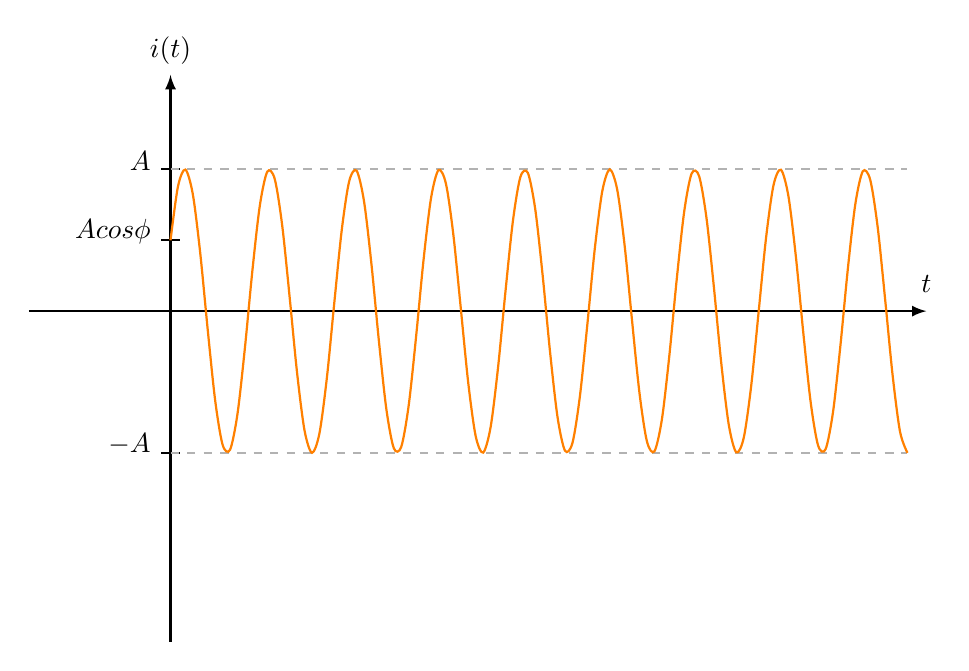
\begin{tikzpicture}[>=latex, thick, scale=1.2]
			% Definizioni per personalizzare il grafico
			\def\A{1.5}
			\def\Phi{-60}
			\def\omega{400}
			
			% --- Assi ---
			% Asse orizzontale (Tempo t)
			\draw[->] (-1.5, 0) -- (8, 0) node[right, above = 3 pt] {$t$};
			% Asse verticale (Corrente i_L(t))
			\draw[->] (0, -3.5) -- (0, 2.5) node[above] {$i(t)$};
			
			% --- Etichette ---
			
			\draw (0.1, {\A * cos(\Phi)}) -- (-0.1, {\A * cos(\Phi)}) node[above=3pt,left] {$Acos\phi$};
			\draw (0.1, {\A}) -- (-0.1,{\A}) node[above=3pt,left] {$A$};
			\draw (0.1, {-\A}) -- (-0.1,{-\A}) node[above=3pt,left] {$-A$};
			
			% --- Curva ---
			
			\draw[black!30,  thick, domain=0:7.8, samples=100, dashed] 
			plot (\x, {\A});
			\draw[black!30,  thick, domain=0:7.8, samples=100, dashed] 
			plot (\x, {-\A});
			\draw[orange,  thick, domain=0:7.8, samples=100, smooth] 
			plot (\x, {\A * cos(\omega *\x + \Phi)});
		\end{tikzpicture}
		\label{fig:nonsmorzata}
		\caption{}
	\end{figure}
\end{enumerate}
Per ricapitolare, osserviamo gli andamenti delle quattro risposte a confronto in \cref{fig:rlcslriassunto}, ottenute mantenendo la stessa $\omega_0$ e facendo variare $\alpha$ come descritto nella legenda.
Osserviamo in particolare la differente altezza dei picchi, e il fatto che la risposta sottosmorzata è quella che porta all'assestamento più velocemente\footnote{Per quanto alla nota precedente, in questo caso la risposta sottosmorzata entra più rapidamente in una generica fascia di tolleranza arbitraria, valutabile visivamente, in quanto si è selezionato un valore di $\zeta = 0.85$, adatto a mostrare il decadimento iniziale rapido, anche se questo non mostra la natura oscillatoria della risposta}
\begin{figure}
	\centering
	\includegraphics[width=0.9\linewidth]{rlcriassunto}
	\caption{}
	\label{fig:rlcslriassunto}
\end{figure}


\subsubsection{RLC serie - Evoluzione forzata}
Facciamo riferimento a \cref{fig:rlcsf}, con regime stazionario con interruttore aperto per $t=0^-$, chiusura dell'interruttore per $t=0$, transitorio per $t\geq 0$
\begin{figure}[H]
	\centering
	\includegraphics[width=0.7\linewidth]{rlcsf}
	\caption{}
	\label{fig:rlcsf}
\end{figure}
Con calcoli analoghi a quelli svolti nel caso dell'evoluzione libera,
\[LKT:\ v_R(t) + v_L(t) + v_C(t) = V_g\]
Utilizzando le leggi costitutive e notando che la corrente che attraversa i tre componenti, collegati in seri, è la stessa $i(t) = i_C(t) = C\frac{dv_C}{dt}$,
\[RC\frac{dv_C}{dt} + LC\frac{d^2i}{dt^2} + v_C(t)= V_g\]
\begin{equation}\label{eq:rlc1}
	\frac{d^2v_C}{dt^2} + \frac{R}{L}\frac{dv}{dt} + \frac{1}{LC} v_c(t) = V_g
\end{equation}
Notiamo quindi che la forma è la stessa dell'\cref{eq:rlc}, in cui però l'incognita è $v_C(t)$ anziché $i(t)$, e l'\cref{eq:rlc1} non è omogenea.
Sfruttiamo la linearità del circuito, quindi scomponiamo la risposta completa in una risposta transitoria $v_{C,t} (t)$ e una a regime $v_{C,r}$:
\[v_C(t) = v_{C,t}(t) + v_{C,r}\]
Per la risposta transitoria,
\[\frac{d^2v_C}{dt^2} + \frac{R}{L}\frac{dv}{dt} + \frac{1}{LC}v_c(t) = 0\]
che è esattamente identica nella forma all'\cref{eq:rlc}.
Dunque, in base alla presenza dei componenti R, L, C, il circuito può avere una risposta transitoria di uno dei quattro tipi già descritti sopra.
\begin{enumerate}
	\item $\Delta > 0$ (\textit{Risposta sovrasmorzata});
	\item $\Delta = 0$ (\textit{Risposta smorzata critica});
	\item $\Delta < 0$ con $\alpha > 0$ (\textit{Risposta sottosmorzata});
	\item $\Delta < 0$ con $\alpha = 0$ (\textit{Risposta senza smorzamento}).
\end{enumerate}

Rimangono da determinare soltanto i parametri $A_1,\ A_2$, dipendenti dalle condizioni iniziali:
\begin{enumerate}
	\item $v_C(0^+) = v_C (0^-) = V_0$
	\item $\left. \frac{dv_C}{dt} \right |_{0^+}$, la quale deve essere ricavata dallo studio del circuito a $t = 0^+$, similmente a quanto fatto per la corrente nel circuito in evoluzione libera. Sostituiamo dunque il condensatore con un generatore di tensione $V_0$ e l'induttore con un generatore di corrente $I_0$. Dal circuito così ottenuto è poi possibile determinare il valore di $\left. \frac{dv_C}{dt} \right |_{0^+}$ sfruttando il fatto che $\frac{dv_c}{dt} = Ci_C$.
\end{enumerate}
Per determinare la risposta a regime, è sufficiente, poi, effettuare un'analisi del circuito in regime stazionario a $t=\infty$, considerando che gli induttori sono equivalenti a cortocircuiti e i condensatori a rami aperti (\cref{fig:rlcsf1}).
\begin{figure}[H]
	\centering
	\includegraphics[width=0.7\linewidth]{rlcsf1}
	\caption{}
	\label{fig:rlcsf1}
\end{figure}
\[LKT: v_C(\infty) = V_g - v_R(\infty) = V_g + Ri_R = V_g\]
Osserviamo nel grafico in \cref{fig:rlcsfriassunto} l'andamento della risposta completa nel tempo in base a diversi valori della resistenza, dunque di $\alpha$ del circuito.
\begin{figure}[H]
	\centering
	\includegraphics[width=0.9\linewidth]{rlcsfriassunto}
	\caption{}
	\label{fig:rlcsfriassunto}
\end{figure}
Siccome la forma delle soluzioni alle equazioni differenziali è la stessa per tutti i circuiti, nella risoluzione degli esercizi è soltanto necessario determinare i valori iniziali e finali (tramite l'analisi a \textit{istanti strategici}) per ottenere la soluzione specifica. Gli esercizi proposto sono dunque studi semplificati di transitori.
\begin{ex}[Studio semplificato di un transitorio]
	Si consideri il circuito in \cref{fig:exrlc}
	\begin{figure}[H]
		\centering
		\begin{circuitikz}
		
		% Definisci le coordinate dei nodi principali
		\coordinate (A) at (0, 0);     % Angolo in basso a sinistra
		\coordinate (D) at (0, 3);     % Angolo in alto a sinistra
		\coordinate (C_split) at (4, 3);   % Punto di diramazione superiore (per R2/Switch)
		\coordinate (C_end) at (6, 3);     % Punto di diramazione superiore (per C)
		\coordinate (B_split) at (4, 0);   % Punto di diramazione inferiore (per R2/Switch)
		\coordinate (B_end) at (6, 0);     % Punto di diramazione inferiore (per C)
		\coordinate (E) at (4, 1.5);       % Nodo intermedio per R2/switch
		
		% 1. Branca di Sinistra (Generatore)
		\draw (A) to[V, v<=$V_g$] (D);
		
		% 2. Branca Superiore (R1 e L)
		\draw (D) to[R, l_=$R_1$] (2, 3)
		to[L, l=$L$] (C_split); 
		
		% 3. Linea superiore di collegamento
		\draw (C_split) -- (C_end);
		
		% 4. Branca Centrale (R2 e Interruttore)
		
		% Resistenza R2
		\draw (C_split) to[R, l_=$R_2$, -*] (E);
		
		% INTERRUTTORE COMPATIBILE: Usiamo 'switch'
		\draw (E) to [switch, l_={$t=0$}] (B_split); 
		
		% Aggiungi l'etichetta della corrente manualmente (per compatibilità)
		\node at (4.5, 0.75) {$i(t)$};
		
		% Aggiungi la freccia per l'azione di chiusura del circuito (come nel disegno a mano)
		%\draw[->] (3.8, 1.2) arc (270:315:0.5); 
		
		% 5. Branca di Destra (C) - ORA SEPARATA
		\draw (C_end) to[C, l=$C$] (B_end); 
		
		% 6. Linea inferiore di collegamento (chiusura del circuito)
		\draw (B_split) -- (A);
		\draw (B_split) -- (B_end); % Collega le basi dei rami paralleli
		\end{circuitikz}
		\caption{}
		\label{fig:exrlc}
	\end{figure}
	
	Si determinino: $i_L(0^-)$,$i_C(0^-)$, $\left. \frac{di_L}{dt}\right|_{0^+}$, $\left. \frac{dv_c}{dt}\right|_{0^+}$, $E_L (\infty)$, $E_L (\infty)$.
	Iniziamo studiando il circuito a $t= 0^-$, con interruttore chiuso, in regime stazionario. Il circuito si semplifica come in \cref{fig:exrlc1}
	\begin{figure}[H]
		\centering
		\begin{circuitikz}
		% --- Coordinate ---
		\coordinate (A) at (0,0);     % Massa sinistra
		\coordinate (B) at (0,3);     % Alto sinistra
		\coordinate (C) at (3,3);     % Nodo dopo R1
		\coordinate (D) at (5,3);     % Nodo sopra R2
		\coordinate (E) at (5,0);     % Nodo sotto R2
		\coordinate (F) at (7,3);     % Terminale aperto alto
		\coordinate (G) at (7,0);     % Terminale aperto basso
		
		% --- 1. Generatore e R1 ---
		\draw (A) to[V, l=$V_g$] (B);
		\draw (B) to[R, l=$R_1$] (C);
		
		% --- 2. Induttore (come Corto Circuito) ---
		% Disegno un filo (short) con due pallini (*-*) per evidenziare che lì c'era L
		\draw (C) to[short, *-*, i=$i_L$] (D);
		% NOTA: Se "i=$i_L$" ti da errore, cancellalo e usa la riga sotto:
		% \node at (4, 3.5) {$i_L \rightarrow$};
		
		% --- 3. Ramo Centrale (R2) ---
		% Uso v=... per la tensione. Se da errore, usa i nodi manuali.
		\draw (D) to[R, l=$R_2$, v=$v_{R2}$] (E);
		
		% --- 4. Ramo di Destra (Condensatore come Circuito Aperto) ---
		\draw (D) -- (F); % Filo superiore
		\draw (E) -- (G); % Filo inferiore
		
		% "open" crea uno spazio vuoto, "o-o" mette i cerchietti dei terminali
		\draw (F) to[open, v=$v_C$, o-o] (G);
		
		% --- 5. Chiusura del circuito (massa) ---
		\draw (E) -- (A);
		
		\end{circuitikz}
		\caption{}
		\label{fig:exrlc1}
	\end{figure}
	\[i_L(0^-) = \frac{V_g}{R_1 + R_2}\]
	\[v_C(0^-) = R_2 i_{R_2} = R_2 \frac{V_g}{R_1 + R_2}\]
	Studiamo il circuito a $t = 0^+$. Per le proprietà di continuità, analogamente a quanto osservato nella teoria precedente, possiamo considerare i componenti dinamici come generatori indipendenti, mantenendo i VDR scelti in precedenza (\cref{fig:exrlc2}).
	
	\begin{figure}[H]
		\centering
		\begin{circuitikz}
			
			% --- Coordinate ---
			\coordinate (A) at (0,0);
			\coordinate (D) at (0,4);
			\coordinate (NodeL) at (4,4);    % Nodo sopra R2
			\coordinate (NodeR) at (8,4);    % Nodo sopra Generatore equiv C
			\coordinate (GndL) at (4,0);     % Nodo sotto R2
			\coordinate (GndR) at (8,0);     % Nodo sotto Generatore equiv C
			
			% --- 1. Generatore Vg (Sinistra) ---
			\draw (A) to[V, l=$V_g$] (D);
			
			% --- 2. Ramo Superiore: R1 e Generatore di Corrente (ex Induttore) ---
			% Nota: I generatori di corrente si indicano con 'isource' (o 'I' nelle vecchie versioni)
			\draw (D) to[R, l=$R_1$] (2,4)
			to[isource, l=$\frac{V_g}{R_1+R_2}$] (NodeL);
			
			% --- 3. Ramo Centrale: R2 e Interruttore Aperto ---
			% Disegno l'interruttore esplicitamente aperto per chiarezza
			\draw (NodeL) to[R, l=$R_2$] (4,2.5);
			\draw (4,2.5) to[open, o-o] (4,1.5); % Spazio vuoto con terminali (switch aperto)
			\draw (4,1.5) -- (GndL);
			
			% --- 4. Ramo Destro: Generatore di Tensione (ex Condensatore) ---
			\draw (NodeL) -- (NodeR);
			
			% Uso 'V' per il generatore che sostituisce C.
			% \displaystyle serve a rendere la frazione leggibile e grande
			\draw (NodeR) to[V, l=$R_2 \frac{V_g}{R_1+R_2}$] (GndR);
			
			\draw (GndR) -- (GndL) -- (A);
		\end{circuitikz}
		\caption{}
		\label{fig:exrlc2}
	\end{figure}
	\[\left. \frac{dv_c}{dt} \right |_{0^+} = \frac{i_C}{C} = \frac{i_L}{C} = \frac{1}{C}\frac{V_g}{R_1 + R_2}\ (V\cdot s^{-1})\]
	\[\left. \frac{di_L}{dt} \right |_{0^+} = \frac{v_L}{L} = \frac{ V_g - v_R - v_C}{L} = \frac{V_g}{L} \left( 1 - \frac{R_1}{R_1 + R_2} -\frac{R_2}{R_1 + R_2} \right) = 0\]
	Studiamo il circuito a $t = \infty$ (\cref{fig:exrlc3}).
	\begin{figure}[H]
		\centering
		\begin{circuitikz}% Aumento leggermente la scala per chiarezza
			
			% Definizione delle coordinate principali per facilitare il disegno
			\coordinate (A_bot) at (0,0); % Angolo in basso a sinistra
			\coordinate (A_top) at (0,3); % Angolo in alto a sinistra
			\coordinate (B_top) at (4,3); % Nodo di giunzione superiore centrale
			\coordinate (B_mid) at (4,1.5); % Punto intermedio nel ramo centrale
			\coordinate (B_bot) at (4,0); % Nodo di giunzione inferiore centrale
			\coordinate (C_top) at (7,3); % Angolo in alto a destra
			\coordinate (C_bot) at (7,0); % Angolo in basso a destra
			
			% --- Ramo di Sinistra e Superiore (Generatore, R1, L) ---
			% Disegno dal basso a sinistra, salgo col generatore, poi a destra con R1 e L
			\draw (A_bot) to[V, l=$V_g$] (A_top)
			to[R, l=$R_1$] (2,3) % Punto intermedio per spaziare R1 e L
			to[L, l=$L$] (B_top);
			
			% --- Ramo Centrale (R2 e Interruttore) ---
			% Parto dal nodo superiore centrale (B_top) e scendo.
			% Uso '*-' per mettere il pallino di giunzione all'inizio.
			\draw (B_top) to[R, l=$R_2$, *-] (B_mid)
			% 'opening switch' disegna la freccia di apertura.
			% Aggiungo l'etichetta t=0.
			to[nos, l={$t=\infty$}] (B_bot);
			
			% --- Ramo di Destra (Condensatore) ---
			% Continuo il filo superiore da B_top a C_top, poi scendo col condensatore.
			\draw (B_top) -- (C_top)
			to[C, l=$C$] (C_bot);
			
			% --- Chiusura del circuito inferiore ---
			% Collego i punti inferiori per chiudere la massa.
			% Uso '-*' per aggiungere il pallino di giunzione sotto l'interruttore.
			\draw (C_bot) -- (B_bot) to[short, -*] (A_bot);
		\end{circuitikz}
		\caption{}
		\label{fig:exrlc3}
	\end{figure}
	
	\[E_L(\infty) = \frac{1}{2}Li_L^2(\infty) = \frac{1}{2}L\left(\frac{V_g}{R_1}\right)^2 \]
	\[E_C(\infty) = \frac{1}{2}Cv_C^2(\infty) = \frac{1}{2}C(Ri_{R_2}(\infty))^2 = 0 \]
\end{ex}
\subsubsection{RLC parallelo - Evoluzione forzata}
Analizziamo un circuito RLC parallelo, direttamente in evoluzione forzata. Da questa trattazione, poi, è possibile ricavare come caso particolare l'evoluzione libera.
Consideriamo, ad esempio, un circuito come in \cref{fig:rlcp}, che rappresenta il caso realistico in cui il transitorio è innescato dalla chiusura di un interruttore. Altri scenari possibili potrebbero essere più complicati.
\begin{figure}[H]
	\centering
	\begin{circuitikz}
		% --- Definisco le coordinate per chiarezza ---
		\coordinate (A_bot) at (0,0);  % Basso Sinistra
		\coordinate (A_top) at (0,3);  % Alto Sinistra (sopra Ig)
		\coordinate (B_top) at (3,3);  % Nodo sopra R
		\coordinate (B_bot) at (3,0);  % Nodo sotto R
		\coordinate (C_top) at (6,3);  % Nodo sopra L
		\coordinate (C_bot) at (6,0);  % Nodo sotto L
		\coordinate (D_top) at (8,3);  % Nodo sopra C
		\coordinate (D_bot) at (8,0);  % Nodo sotto C
		
		% --- Parte Sinistra: Generatore Ig e Resistenza R ---
		% Disegno il generatore di corrente (I) che sale
		\draw (A_bot) to[I, l=$I_g$] (A_top);
		
		% Collega la parte superiore e disegna la resistenza R
		\draw (A_top) -- (B_top)
		to[R, l=$R$, *-*] (B_bot) % *-* mette i pallini ai nodi
		-- (A_bot); % Chiude il loop in basso
		
		% --- Parte Centrale: Interruttore ---
		% 'closing switch' disegna l'interruttore aperto con la freccia che chiude
		\draw (B_top) to[closing switch] (C_top);
		
		% --- Parte Destra: Induttore L e Condensatore C ---
		% Disegno l'induttore L
		\draw (C_top) to[L, l=$L$, *-*] (C_bot);
		
		% Collega il condensatore C in parallelo
		\draw (C_top) -- (D_top)
		to[C, l=$C$] (D_bot)
		-- (C_bot);
		
		% --- Collegamento di massa inferiore ---
		% Unisce la massa di sinistra con quella di destra
		\draw (B_bot) -- (C_bot);
	\end{circuitikz}
	\caption{}
	\label{fig:rlcp}
\end{figure}
Applichiamo lo stesso metodo già utilizzato per RLC serie per indagare il comportamento del circuito per $t \geq 0$, durante il transitorio.

\[LKC:\ i_R(t) + i_L(t) + i_C(t) = I_g\]
\[\frac{v(t)}{R} + i_L(t) + C\frac{dv}{dt} = I_g\]
\[\frac{L}{R} \frac{di_L}{dt} + i_L(t) + C\frac{d^2i_L}{dt} = I_g\]

\begin{equation} \label{eq:rlcp}
	\frac{d^2i_L}{dt} + \frac{1}{RC} \frac{di_L}{dt} + \frac{1}{LC} i_L(t) = \frac{1}{LC}I_g
\end{equation}
Notiamo che l'\cref{eq:rlcp} è molto simile all'\cref{eq:rlc1}, con l'unica differenza che in questo caso è la tensione la funzione incognita. In questo caso, $\omega_0$ ha lo stesso valore in funzione dei parametri del sistema ($\omega_0 = \frac{1}{\sqrt{LC}}$), mentre $\alpha = \frac{1}{2RC}$.
Dunque anche in questo caso il polinomio caratteristico è 
\[\lambda^2 + 2 \alpha \lambda + \omega_0^2 = 0\]
\[\lambda_{1,2} = -\alpha \pm \sqrt{\Delta},\quad \Delta = \alpha^2 - \omega_0^2\]
Siccome il circuito è lineare, possiamo leggere la risposta completa come somma di una risposta transitoria e una regime:
\[i_L(t) = i_{L,t} (t) + i_{L,R}\]
La risposta transitoria può avere le forme già descritte sopra:
\begin{enumerate}
	\item $\Delta > 0$, \textit{Risposta sovrasmorzata};
	\item $\Delta = 0$, \textit{Risposta smorzata critica};
	\item $\Delta < 0$ con $\alpha > 0$, \textit{Risposta sottosmorzata};
	\item $\Delta < 0$ con $\alpha = 0$, \textit{Risposta senza smorzamento}.
\end{enumerate}
I parametri $A_1,\ A_2$ dipendono dalle condizioni iniziali, $i_L(0^+) = i_L(0^-)$; $\left. \frac{di_L}{dt} \right |_{0^+}$, che può essere ottenuta analizzando il circuito all'istante iniziale, considerando i componenti dinamici come generatori indipendenti per quell'istante, in modo del tutto analogo a quanto sopra.\\
Per determinare la risposta a regime, consideriamo il circuito per $t = \infty$, a transitorio concluso (\cref{fig:rlcp1}). Dunque, banalmente,
\[i_{L,R} = I_g\]
\begin{figure}[H]
	\centering
	\begin{circuitikz}[american]
		% Coordinate
		\coordinate (A_bot) at (0,0);
		\coordinate (A_top) at (0,3);
		\coordinate (B_top) at (3,3);
		\coordinate (B_bot) at (3,0);
		\coordinate (C_top) at (6,3);
		\coordinate (C_bot) at (6,0);
		\coordinate (D_top) at (9,3);
		\coordinate (D_bot) at (9,0);
		
		% 1. Generatore di Corrente Ig
		\draw (A_bot) to[I, l=$I_g$] (A_top);
		
		% 2. Resistenza R (che viene cortocircuitata)
		% Aggiungo i_R verso il basso
		\draw (A_top) -- (B_top);
		\draw (B_top) to[R, l=$R$, i>=$i_R$] (B_bot);
		
		% (Opzionale) Se vuoi disegnare la barra trasversale che indica che è esclusa:
		%\draw[thick] (2.5, 0.5) -- (3.5, 2.5); 
		
		% 3. Induttore -> Corto Circuito (Filo)
		% Uso *-* per mostrare i nodi pieni come nel disegno
		\draw (B_top) -- (C_top);
		\draw (C_top) to[short, *-*, v=$v_L{=}0$] (C_bot);
		
		% 4. Condensatore -> Circuito Aperto
		% Uso o-o per i terminali aperti
		\draw (C_top) -- (D_top);
		\draw (D_top) to[open, o-o, v=$v_C$, i=$i_C{=}0$] (D_bot);
		
		% Collegamenti inferiori (Massa)
		\draw (A_bot) -- (D_bot);
	\end{circuitikz}
	\caption{}
	\label{fig:rlcp1}
\end{figure}
Perciò, gli andamenti possibili per la risposta $i_L(t) = i_{L,t}(t) + I_g$ sono rappresentati in \cref{fig:rlcp2}.
\begin{figure}[H]
	\centering
	\includegraphics[width=0.8\linewidth]{rlcp2}
	\caption{}
	\label{fig:rlcp2}
\end{figure}
Nel grafico, generato per opportuni valori delle condizioni iniziali adatti a mostrare la stretta analogia, notiamo, come previsto la totale somiglianza degli andamenti con quelli graficati in \cref{fig:rlcsfriassunto}.\\
Omettiamo per semplicità lo studio delle altre variabili del circuito, che possono essere semplicemente determinati tramite le leggi di Kirchhoff.

\subsection{Calcolo delle costanti $A_1$ e $A_2$}
Il calcolo è analogo per tutti i casi. Prendendo, ad esempio, il caso della risposta sovrasmorzata, esse possono essere ricavate dal seguente sistema di due equazioni in due incognite, dove i valori di $x(t)$ e della sua derivata possono essere determinati per ispezione diretta, come mostrato sopra.
\[\begin{cases}
	x(t) = A_1 e^{\lambda_1 t} + A_2 e^{\lambda_2 t}\\
	\frac{dx}{dt} = \lambda_1 A_1 e^{\lambda_1 t} + \lambda_2 A_2 e^{\lambda_2 t}
\end{cases}\]
Per semplificare i calcoli, siccome $A_1$ e $A_2$ sono costanti, possiamo studiare il sistema per $t=0^+$, e usare i necessari valori dall'ispezione del circuito, come anticipato sopra:
\[\begin{cases}
	x(0^+) = A_1 + A_2 \\
	\left. \frac{dx}{dt} \right |_{0^+} = \lambda_1 A_1 + \lambda_2 A_2
\end{cases}\]
\[\begin{cases}
	A_1 = x(0^+) - A_2\\
	\left. \frac{dx}{dt} \right |_{0^+} = \lambda_1 x(0^+) - \lambda_1 A_2 + \lambda_2 A_2 = \lambda_1 x(0^+) + A_2 (\lambda_2 \lambda_1)
\end{cases}\]
\[\begin{cases}
	A_1 = \frac{\left. \frac{dx}{dt} \right |_{0^+} - \lambda_2 x(0^+)}{\lambda_1 - \lambda_2}
	A_2 = \frac{\left. \frac{dx}{dt} \right |_{0^+} - \lambda_1 x(0^+)}{\lambda_2 - \lambda_1}\\
\end{cases}\]
Per le altre forme, si ottengono forme analoghe (non identiche, in quanto la forma di partenza è differente).

\subsection{Risonanza}
\subsubsection{Risonanza - RLC serie}
Esploriamo in questa sezione il concetto di \textit{risonanza} in un circuito RLC.\\
Consideriamo un ramo di un circuito RLC serie in regime sinusoidale, come in \cref{fig:risonanza}, e indaghiamone il comportamento al variare della frequenza $\omega$ di oscillazione della tensione nel circuito.

\begin{figure}[H]
	\centering
	\begin{circuitikz}[american]
		% Coordinate
		\coordinate (In_Bot) at (0,0);
		\coordinate (In_Top) at (0,3);
		\coordinate (Top_Right) at (4,3);
		\coordinate (Bot_Right) at (4,0);
		
		% --- MODIFICA QUI ---
		% Disegno da SOPRA a SOTTO per avere il + in alto.
		% Uso '<' per girare la freccia verso l'alto.
		% Uso '^' (opzionale) per spostare l'etichetta se si sovrappone
		\draw (In_Top) to[open, v^>=$\underline{V}$, o-o] (In_Bot);
		% --------------------
		
		% Ramo Superiore
		\draw (In_Top) to[short, i=$\underline{I}$] (1,3) 
		to[generic, l=$\underline{Z}_R$] (Top_Right);
		
		% Ramo Destro
		\draw (Top_Right) to[generic, l=$\underline{Z}_L$] (Bot_Right);
		
		% Ramo Inferiore
		\draw (Bot_Right) to[generic, l=$\underline{Z}_C$] (In_Bot);
		
	\end{circuitikz}
	\caption{}
	\label{fig:risonanza}
\end{figure}

\[\underline{Z} = Z_R + \underline{Z_L} + \underline{Z_C} = R + j \omega L - \frac{j}{\omega C} = R + jX\]
\[X(\omega) = \omega L - \frac{1}{\omega C}\]
Notiamo che la reattanza del sistema, all'aumentare della frequenza, ha un termine che aumenta e uno che diminuisce. Ci chiediamo dunque se esista un valore $\omega_0$ tale da annullare la reattanza:
\[\omega_0 L - \frac{1}{\omega_0 C} \Leftrightarrow \omega_0 = \frac{1}{\sqrt{LC}}\]
Notiamo che questo valore è proprio quello che abbiamo impiegato come \textit{frequenza di risonanza} nella descrizione dei transitori. Questa è l'origine del termine: per $\omega = \omega_0$, il circuito si dice operante in condizione di risonanza, e
\[\underline{Z} = R + j0 = R\]
L'interesse per questo circuito è legato alle proprietà dell'andamento della corrente che scorre nel circuito al variare della frequenza.\\
\begin{center}
	% 2. Aumenta l'altezza delle righe (2 volte il normale)
	\renewcommand{\arraystretch}{2.5}
	
	% 3. Aumenta lo spazio laterale nelle celle (padding orizzontale)
	\setlength{\tabcolsep}{25pt}
	\begin{tabular}{c|c|c}
		
		\textbf{$\omega$} &\textbf{$X$} & \textbf{$\displaystyle \underline{I}=\frac{\underline{V}}{\sqrt{R^2 + X^2}}$}\\ % Intestazione della tabella in modalità matematica
		\hline % Linea orizzontale sotto l'intestazione
		$0$ & $\displaystyle \lim_{\omega \to 0} \left( \omega L - \frac{1}{\omega C} \right) = 0 - \infty = -\infty$ & $0$ \\ % Contenuto della riga con formula complessa
		
		$\omega_0$ & $0$ & $\frac{V}{R}$\\
		 
		$\infty$ & $\infty$ & $0$\\
	\end{tabular}\\
\end{center}
Ci aspettiamo dunque un andamento della corrente che esibisca un picco alla frequenza di risonanza e tenda a 0 a $\omega = \pm \infty$. Tale picco sarà più alto tanto più piccola la resistenza. Per una resistenza nulla, si avrebbe un comportamento asintotico: se non opportunamente limitato, la corrente tenderà all'infinito (\cref{fig:risonanza1}). All'atto pratico, salirà fino al limite di protezione del generatore utilizzato, imposto dai produttori per evitare danni irreversibili ai circuiti interni e collegati.\\
\begin{figure}[H]
	\centering
	\includegraphics[width=0.7\linewidth]{risonanza1}
	\caption{}
	\label{fig:risonanza1}
\end{figure}

Analizziamo anche l'andamento di $\varphi = \varphi(\omega) = arg(\underline{Z})$.\\
\begin{center}
	\renewcommand{\arraystretch}{2.5}
	
	% 3. Aumenta lo spazio laterale nelle celle (padding orizzontale)
	\setlength{\tabcolsep}{25pt}
	\begin{tabular}{c|c}
		\textbf{$\omega$} & \textbf{$\varphi = arg(\underline{Z}) = atan(\frac{X}{R})$}\\ % Intestazione della tabella in modalità matematica
		\hline % Linea orizzontale sotto l'intestazione
		$0$ & $atan{-\infty} = -\frac{\pi}{2}$\\ % Contenuto della riga con formula complessa
		
		$\omega_0$ & $atan(0) = 0$\\
		 
		$\infty$ & $atan{\infty} = \frac{\pi}{2}$
	\end{tabular}\\
\end{center}


Notiamo dunque che lo sfasamento dovrà avere un andamento analogo a quello della funzione arcotangente, con radice in $\omega_0$. A basse frequenze ($\omega < \omega_0$), il circuito è dominato dal comportamento capacitivo; al contrario, alle alte frequenze ($\omega > \omega_0$), dal comportamento induttivo. Per $\omega 0 \omega_0$, il comportamento è ohmico, puramente resistivo, con corrente e tensione in fase (\cref{fig:risonanza2}). Questo deve essere tenuto in considerazione per ottenere il comportamento desiderato da induttori e capacitori in regime sinusoidale.
\begin{figure}[H]
	\centering
	\includegraphics[width=0.7\linewidth]{risonanza2}
	\caption{}
	\label{fig:risonanza2}
\end{figure}

\subsubsection{Antirisonanza - RLC parallelo}
\begin{figure}[H]
	\centering
	\begin{circuitikz}[american]
		% Coordinate
		\coordinate (In_Top) at (0,3);
		\coordinate (In_Bot) at (0,0);
		\coordinate (Node_Top) at (3,3); % Nodo sopra il parallelo
		\coordinate (Node_Bot) at (3,0); % Nodo sotto il parallelo
		\coordinate (Par_Right_Top) at (5,3);
		\coordinate (Par_Right_Bot) at (5,0);
		
		% 1. Tensione V (+ sopra, - sotto, freccia in su)
		% Disegno da SOPRA (In_Top) a SOTTO (In_Bot) -> Il '+' va alla partenza (sopra).
		% Uso '<=' per invertire la freccia (farla puntare verso l'alto).
		\draw (In_Top) to[open, v<=$\underline{V}$, o-o] (In_Bot);
		
		% 2. Ramo Serie: Corrente I e Resistenza R
		% Uso un piccolo tratto 'short' per la corrente, poi la Resistenza
		\draw (In_Top) to[short, i=$\underline{I}$] (1,3) 
		to[R, l=$R$] (Node_Top);
		
		% 3. Parallelo - Ramo Sinistro (Simbolo C, Label L)
		% Nota: Nel tuo disegno questo componente ha il simbolo del condensatore (C)
		% ma l'etichetta 'L'. Ho rispettato il disegno.
		\draw (Node_Top) to[C, l=$L$] (Node_Bot);
		
		% 4. Parallelo - Ramo Destro (Simbolo L, Label C)
		% Collega a destra, scende con l'induttore, torna a sinistra
		\draw (Node_Top) -- (Par_Right_Top)
		to[L, l=$C$] (Par_Right_Bot)
		-- (Node_Bot);
		
		% 5. Chiusura del circuito (linea di fondo)
		\draw (Node_Bot) -- (In_Bot);
		
	\end{circuitikz}
	\caption{}
	\label{fig:risonanza3}
\end{figure}
Consideriamo il circuito in \cref{fig:risonanza3}, e proseguiamo con considerazioni analoghe.
\[\underline{Z} = R + jX = \frac{j\omega L \cdot (-\frac{j}{\omega C})}{j\omega L - \frac{j}{\omega C}} = - j \frac{\frac{L}{C}}{\omega L - \frac{1}{\omega C}} \]
Dunque, 
\[X(\omega) = - \frac{\frac{L}{C}}{\omega L - \frac{1}{\omega C}} \] 
Osserviamo che non esiste alcun valore di $omega$ che annulla la reattanza. Osserviamo, anzi, che la reattanza tende a infinito per $omega = \omega_0$:
\[X(\omega_0) = -\frac{\frac{L}{C}}{0}\]
\begin{center}
	% 2. Aumenta l'altezza delle righe (2 volte il normale)
	\renewcommand{\arraystretch}{2.5}
	
	% 3. Aumenta lo spazio laterale nelle celle (padding orizzontale)
	\setlength{\tabcolsep}{25pt}
	\begin{tabular}{c|c}
		
		\textbf{$\omega$} & \textbf{$X$}\\ % Intestazione della tabella in modalità matematica
		\hline % Linea orizzontale sotto l'intestazione
		$0$ & $0$ \\ % Contenuto della riga con formula complessa
		
		$\omega_0^-$ & $\infty$\\
		
		$\omega_0^+$ & $- \infty$\\
		
		$\infty$ & $0$\\
	\end{tabular}\\
\end{center}
L'andamento della reattanza è quindi quello rappresentato in \cref{fig:risonanza4}, che ha comportamento duale a quello della risonanza: si ha comportamento ohmico-induttivo per basse frequenze e ohmico-capacitivo ad alte frequenze. Le correnti tendono ad annullarsi in prossimità della pulsazione di antirisonanza.\\
\begin{figure}[H]
	\centering
	\includegraphics[width=0.7\linewidth]{risonanza4}
	\caption{}
	\label{fig:risonanza4}
\end{figure}
Notiamo che per $\omega = 0$, il parallelo RC è visto come un cortocircuito, con $\underline{Z_L} = 0$ e $\underline{Z_C} = \infty$ e tutta la corrente scorre sull'induttore, che si comporta come un circuito aperto, mentre il condensatore come un cortocircuito.\\
Per $\omega = \infty$, il comportamento è perfettamente speculare, con il condensatore che si comporta come cortocircuito e l'induttore come circuito aperto.\\
Per $\omega = \omega_0$, nessuno dei due componenti ha impedenza infinita o nulla, tuttavia il parallelo dei due ha impedenza infinita, e perciò la corrente entrante e uscente dal parallelo è nulla. I due componenti singolarmente sentono la tensione V applicata ai capi del ramo (la caduta sul resistore è nulla perché non scorre corrente). Perciò su essi, nel ramo interno al parallelo in realtà si ha una corrente, e per la LKC $\underline{I_C} = \underline{I_L} = j\underline{V} \omega C = -\frac{j \underline{V}}{\omega L}$, detta \textit{corrente di circolazione}. In fase di progettazione, è dunque necessario verificare che anche questa corrente sia compatibile con le caratteristiche dei componenti, e non rischi di danneggiarli.
